\documentclass[12pt]{article}
\usepackage{graphicx}
\begin{document}

\section*{Random Rug}

First, we consider the probability that a 4x4 rug would be rejected. This would be the equivalent of flipping 16 3-sided coins and having them all come up heads.
\begin{equation}
P_{44} \equiv P(\hbox{rej})_{4x4} = \frac{1}{3^{16}} = 2.32 * 10^{-8}
\end{equation}

Not very likely! But what happens if we make the rug one piece bigger in each dimension? In a 5x5 rug, there are four distinct 4x4 subsections.

\begin{figure}[h]
    \centering
    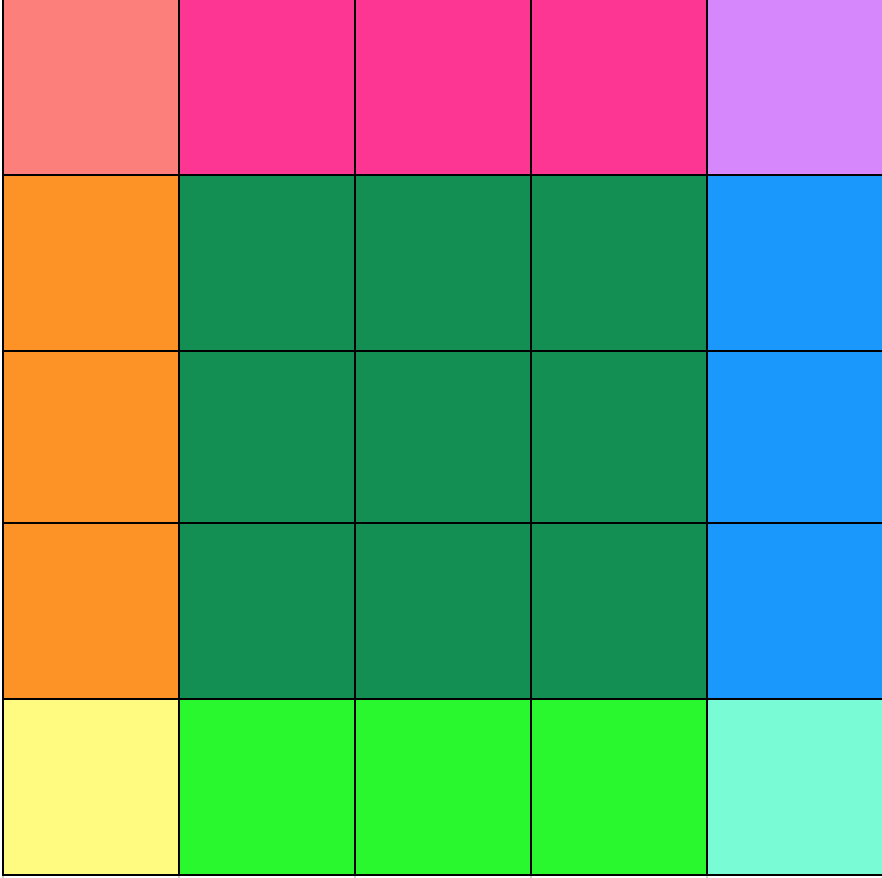
\includegraphics[scale=0.45]{5x5rugs.png}
    \caption{In a 5x5 rug, there are four distinct 4x4 subsections to try. The pure red, magenta, yellow, and cyan squares at the corners belong to exactly one subsection. The edges belong to two subsections, and the middle 3x3 square is shared by all four subsections.}
    \label{fig: four 4x4 subsections of rug}
\end{figure}

Since there are four chances at rejection, we multiply our original probability from equation (1). 

\begin{equation}
P(\hbox{rej})_{5x5} = 4 * P_{44} = 9.29 * 10^{-8}
\end{equation}

Say we define $N_{44}$ is the number of distinct 4x4 grids on a rug. This leads us to a formula like this:
\begin{equation}
P(\hbox{rej}) = N_{44} * P_{44}
\end{equation}

But that relationship doesn't make sense, because once $N_{44}$ becomes quite large\footnote{Specifically, when $N_{44} = \frac{1}{P_{44}}$, or just over 43 million}, $P(\hbox{rej})$ exceeds 1. The probability should converge exactly 1 as $N_{44}$ approaches $\infty$. 

The problem, of course, is that our 4x4 subsections share a lot of real estate, so if something is off anywhere in the 3x3 dark green square from Figure 1, all four subsections will be acceptable. We must account for this.

Might as well start with brute force! We can multiply the following quantities: 
\begin{enumerate}
  \item the probability that the 3x3 center square is all the same color
  \item the probability that a valid combination of the four inner edge strips (hot pink, orange, blue, lime) is also that color
  \item the probability that a corresponding corner piece is also that color
\end{enumerate}

Hm... that doesn't really make sense either, and I don't see how it scales up. "There's got to be a better way."

Brute force, I suppose! Okay, let's instead write a Python script that does the following:

\begin{enumerate}

\item Create a 100x100 grid and fill it with random values 1, 2, 3. 
\item (\textbf{some kind of 4x4 checker algorithm})
\item Record the results 
\item Do this like a million times and see what happens

\end{enumerate}

Yeah, it's not theoretical, but I could answer the question! Now for the algorithm in step 2. It's gotta be quick, ideally. The easiest thing to do would be to treat every square as a potential top left corner and check the 15 below it, stopping if any don't match. Sounds slow and wasteful, with the potential to be looking at 16 billion squares total in the worst case. Well, let's see how slow it is.

The longest trial, which lasted a couple hours, reported this: "TRIALS: 100000; LEGAL RUGS: 99930; ILLEGAL RUGS: 70"


\end{document}